\documentclass[11pt]{article}
\usepackage{parskip}
\usepackage{a4wide}
\usepackage{amsmath}
\usepackage{amsthm}
\usepackage{amsfonts}
\usepackage{amssymb}
\usepackage{fancyhdr}
\usepackage{alltt}
\usepackage{graphicx}
\usepackage[usenames,dvipsnames]{color}
\usepackage[T1]{fontenc}

\newcommand\midtilde{{\lower.50ex\hbox{\texttt{\char`\~}}}}
\newcommand{\term}[1]{\texttt{\color{Cyan}#1}}
\newcommand{\nterm}[1]{\textnormal{\em\color{Brown}#1}}

\pagestyle{fancy}

\begin{document}

\setcounter{secnumdepth}{5}


\title{YAPPL: Yet Another Probabilistic Programming Language}
\author{  David Hu \\ Jonathan Huggins \\ Hans Hyttinen  \\ Harley McGrew}

\maketitle

\fancyhead{}
\fancyhead[L]{}
\fancyhead[C]{YAPPL: Yet Another Probabilistic Programming Language}
\fancyhead[R]{}

\newpage

\tableofcontents

\newpage

\section{ Adminstrative}

Tasks
\begin{itemize}
\item Lexer/Parser
\item Static semantics/Code generation
\item Regression testing
\item Write final document
\end{itemize}

Assignments:
\begin{itemize}
\item David:
\begin{itemize}
\item lexer/parser
\end{itemize}
\item Hans
\begin{itemize}
\item regression tests
\item non-array operators
\end{itemize}
\item Jonathan
\begin{itemize}
\item function evaluation
\item value binding
\end{itemize}
\item Harley
\begin{itemize}
\item arrays
\item pattern matching
\end{itemize}
\end{itemize}

\section{Introduction}
Probabilistic programming languages (PPLs) have grown increasingly popular in the machine learning research in recent years because they allow for the concise definition of complex statistical models. PPLs provide mechanisms for defining generative Bayesian models and conditionally sampling from them. The two key features the PPLs have to accomplish this are conditional evaluation and memoization. Conditional evaluation allows a function to be evaluated conditional on some predicate of its return value being true (this corresponds to conditional sampling from the model). A memoized function remembers what value it returned for previously evaluated argument values and always returns the same value in the future given those arguments. Memoization is useful because it allows elements from ``infinite'' random structures (like lists or matrices) to be generated lazily (as needed). 

YAPPL (Yet Another Probabilistic Programming Language) is inspired primarily inspired by the probabilistic programming language Church, an implementation of a pure subset of Scheme (a dialect of Lisp) for generating models using probabilistic functions. Church relies on the standard Lisp syntax, however, which can be unintuitive and difficult to read. The syntax of YAPPL is inspired by OCaml and contains special constructs for the probabilistic elements of the language, which makes it more approachable and human-readable than Church. In particular, conditional evaluation and memoization are directly built into the YAPPL language. This makes it easier to write and understand the probabilistic models written in YAPPL. 

YAPPL is an almost pure functional programming language. The only functions that produce side-effects are those explicitly built into the language: printing, seeding the random number generator, generating random numbers, and functions defined via memoization. 

We hope YAPPL will serve to demonstrate how writing a PPL from the the ground up can produce that is accessible and useful to a wide audience. 
 


\newpage

\section{Language Tutorial}
YAPPL was designed to make it easy to work with probabilities. The following tutorial will give a quick tour of the basics of the language and eventually build up to define a probability distribution and draw samples from it.

\subsection{Basic variables}

Let's begin by exploring the simple concepts of the language. There are three basic data types: integers, floating-point numbers, and booleans. Here's how to declare variables as each one of these:
\begin{floatbox}
\begin{verbatim}
int:num
float:number_with_a_dot
bool:truthful
\end{verbatim}
\caption{Variable declarations.}
\end{floatbox}

It would be helpful if we could give these variables values and actually use them. To do so, we need to discuss scope. When a variable is bound to a value, you must also specify where it is defined. This is done explicitly through the \texttt{let\dots in} operation:

\begin{floatbox}
\begin{verbatim}
let int:num = 5 in
  num + 5
\end{verbatim}
\caption{Variable definition and scoping.}
\end{floatbox}

The scope of \texttt{num} is the block after \texttt{in}.

\subsection{Functions}

Function declaration and definition looks similar to its variable counterparts. Scoping works in a similar way, though a function's scope begins immediately after the \texttt{=}, so it may be called recursively.  There is no need to explicitly define a function as being recursive. 
\begin{floatbox}
\begin{alltt}
fun int:add int:a int:b = 
   a + b
in 
  {\midtilde}print\_line {\midtilde}add 1 2
\end{alltt}
\caption{A simple function.}
\end{floatbox}

This creates a function \texttt{add} that returns an integer and takes in two integers as arguments. The body of the function is after the \texttt{=} sign. A function returns whatever value its body expression evaluates to. 

Functions are called using the function evaluation operator, tilde (\midtilde). 

\subsubsection{Built-in functions}

The above code also demonstrates a built-in function of YAPPL, \texttt{print\_line}, which takes in a single argument to print. The other built-in functions are \texttt{rand} and \texttt{seed}, which we will use later in this tutorial.

\subsection{Expressions}

Function and variable declarations and definitions are expressions, so are function evaluations. Sequences of expressions are separated by semicolons. The \texttt{if} statement will be useful in this tutorial:
\begin{floatbox}
\begin{alltt}
if x < 10 then
  {\midtilde}print\_line x
else
  {\midtilde}print\_line 10
\end{alltt}
\caption{An \texttt{if} statement.}
\end{floatbox}

For a more formal description, please see the Language Reference Manual. 

\subsection{A simple distribution}

We now know enough to construct a function that takes a sample from a distribution. We will use the geometric distribution because it is a simple enough construct to use in an exemplary program, but still interesting. To remind the reader, a sample from a geometric distribution will return the number of Bernoulli trials needed to obtain a success, given some probability of success $p$. 

Our approach will generate a random number for a number of iterations. Each time a random number is generated, we will increase our integer return value. The function will continue to iterate until the random number is within $[0, p)$. We return the final value. We implement the increment recursively:

\begin{floatbox}
\begin{alltt}
fun int:geom float:p int:i =
    if {\midtilde}rand < p then
      i
    else
      {\midtilde}geom p (i+1)
\end{alltt}
\caption{The basics of sampling from a geometric distribution.}
\end{floatbox}

This is a good start, except we now mention a nuance of YAPPL. For \texttt{rand} to return unique numbers on each execution of a program, \texttt{seed} must first be called. Furthermore, the interface is not very clean: it would be better to have a function that takes a single parameter that is some probability $p$. Finally, we would actually like to call this and run the program. The final code for \texttt{geom.ypl} is below.

\begin{floatbox}
\begin{alltt}
 {\midtilde}seed;
 fun int:geom float:p =
   fun int:geom_helper float:orig_p int:i =
     if {\midtilde}rand < orig_p then
       i
     else
       {\midtilde}geom_helper orig_p (i+1)
   in 
     {\midtilde}geom_helper p 1
 in
   {\midtilde}print_line {\midtilde}geom 0.1
\end{alltt}
\caption{The full \texttt{geom.ypl}.}
\end{floatbox}

\subsection{Compilation and execution}

To compile a YAPPL file, you must pass it into the YAPPL compiler, which will produce an OCaml source file. In order to execute the resulting OCaml code, it will first have to be linked with YAPPL's built-in function library. The following is the basic breakdown of compiling and executing a \texttt{.ypl} file:

\begin{floatbox}
\begin{alltt}
\$ ./yappl < geom.ypl > geom.ml
\$ ocamlc -c geom.ml
\$ ocamlc -o geom unix.cma builtin.cmo geom.cml
\$ ./geom
\$ 8
\end{alltt}
\caption{Compilation and execution.}
\end{floatbox}

%# single line comment
%### multi
%    line
%	comment
%###
%
%# value definition
%float:q = .9;
%# q is defined as 0.9 in the global scope
%
%# sample binding;
%int:x = ~geom q | @ > 5;
%# x is bound to the return value of the function geom evaluated with
%# parameter q; the �| @ > 5� means that the return value of ~geom q is 
%# conditions being greater than 5
%
%# function definition
%int:oneOrTwo float:q = geom q | @ = 1 or @ = 2;
%# a function that samples from geom q, conditional on the sample being 1 or 2
%
%# function equivalent to above
%fun int:oneOrTwo2 int:q =
%   int:x = ~geom q in
%   if x = 1 or x = 2 then
%x
%   else
%~oneOrTwo2 q;
%
%fun bool gtFive int:x = x > 5;
%
%# this is a memoized function
%fun int:f int:n := ~geom .9 | gtFive @;
%~f 0;
%-> 16
%~f 1;
%-> 6
%# later, ~f 0 still returns 16
%~f 0;
%-> 16 
%
%fun int[]:apply (fun int int):f int[]:a =
%	match(a) with
%case x :: rest -> ~f x :: ~apply f rest
%		case [] 	   -> ();
%# apply has type fun int[] ((fun int int) int[])
%# f has type fun int (int)
\newpage

\section{Language Reference Manual}

\subsection{Notation}

Through the document, \nterm{nonterminals} are in brown italics and \term{terminals} are in light blue monospace. Regular expression-like constructs are used to simplify grammar presentation and are in black. Brackets \texttt{[]} are used to indicate optional parts of productions, curly braces \texttt{\{\}} indicate portions of productions that can appear zero or more times, and parentheses \texttt{()} indicate grouping, with a vertical bar \texttt{|} separating options. 

\subsection{Definition of a program}

A program is a sequence of one or more expressions.

\subsection{Lexical conventions}

As syntax of YAPPL is inspired by OCaml, many of the lexical conventions follow those of that language. YAPPL has four kinds of tokens: identifiers, keywords, constants, and expression operators. Whitespace such as blanks, tabs, and newlines are ignored and serve to separate tokens. They have no other semantic meaning. Comments are also ignored.

\subsubsection{Comments}

A single \term{\#} indicates that all succeeding characters shall be considered part of a comment and ignored until a newline is encountered. \\
\\
Immediately following a newline, a series of three \term{\#\#\#} indicates that all succeeding characters shall be considered part of a comment until another series of three \term{\#\#\#} is encountered. Note that newlines are ignored following the \term{\#\#\#}, which essentially delimits multi-line comments.

\subsubsection{Identifiers}

An identifier is a series of alphabetical letters and digits; the first character must be alphabetic. 

\subsubsection{Keywords}

The following identifiers are reserved as keywords/special function and may not be used otherwise:
\begin{table}[htdp]
\center
\begin{tabular}{c c c}
\term{fun} & \term{if} &\term{match} \\
\term{int} & \term{then} & \term{with} \\
\term{bool} & \term{else} &\term{case} \\
\term{float} & \term{in} & \term{string} \\
\term{true} & \term{false} & \term{print} \\
 \term{rand} & \term{and} & \term{or} \\
 \term {given} & \term{print\_line} & \term{seed}
\end{tabular}
\label{default}
\end{table}

The keyword \term{string}  is not currently used, but is reserved for future use.

\subsubsection{Constants}

The reserved boolean constants are \term{true} and \term{false}. The empty list constant is \term{[]} (for all types). 

\subsubsection{Integer Literals}

An integer literal is a sequence of one or more digits, optionally preceded by a minus sign.

Examples of integer literals are \texttt{1337} and \texttt{-42}. 

\subsubsection{Floating-point Literals}

Floating-point decimals consist in an integer part, a decimal part and an exponent part. The integer part is a sequence of one or more digits, optionally preceded by a minus sign. The decimal part is a decimal point followed by zero, one or more digits. The exponent part is the character \texttt e or \texttt E followed by an optional \texttt + or \texttt - sign, followed by one or more digits. The decimal part or the exponent part can be omitted, but not both to avoid ambiguity with integer literals. 

Examples of floating-point constants are \texttt{9000.1}, \texttt{2e-5}, and \texttt{1.4e9}.


\subsection{Types}

The following are the basis data types in YAPPL:\\
\begin{tabular}{l l}
\term{int} & an integer.\\
\term{float} & double-precision floating point.\\
\term{bool} & a boolean value (either \texttt{true} or \texttt{false}).\\
\term{fun} & a function.\\
\end{tabular}\\\\
In addition there are derived array types denoted

\quad \nterm{type} \term{[ ]}


\subsubsection{Non-function Type Declarations}
All bindings must either be declared within a function declaration or declared when bound. A non-function declaration specifies a type and an identifier in the format \nterm{type} \term{:} \nterm{identifier}. Spaces around the colon are optional.  Examples of non-function type declarations:

\begin{alltt}
\quad int:temp
\quad float[]:data
\quad bool : flag
\end{alltt}

\subsubsection{Function Type Declarations}

Function declarations consists of \term{fun} followed by a type declaration for the function in the format \nterm{fun-type} \term{:} \nterm{identifier}. This is followed by zero or more type declarations for arguments of function, which are separated by whitespace. The return types for a function may be a basic type or a function type in the format \term{( fun} \nterm{return-type} \nterm{arg-types} \term{)}

Below are examples of function type declarations: 

\begin{alltt}
\quad fun int:add int:a int:b
\quad fun bool:contains float:a float[]:list
\quad fun (fun int int):fun_gen int:a
\end{alltt}

\subsection{Operations}

\subsubsection{Value binding}

Values are bound to names through the construct 

\begin{alltt}
\quad \nterm{value-decl}\textsuperscript{1} \term{=} \nterm{expr}\textsuperscript{1}  \term{and} \dots \term{and} \nterm{value-decl}\textsuperscript{n} \term{=} \nterm{expr}\textsuperscript{n} \term{in} \nterm{expr}
\end{alltt}

which evaluates  \nterm{expr}\textsuperscript{1} \dots  \nterm{expr}\textsuperscript{n} in the order of declaration and binds the values of those expressions to the names specified in \nterm{value-decl}\textsuperscript{1} \dots \nterm{value-decl}\textsuperscript{n}. The scope of a value declaration begins directly to the right of the declaration.

\subsubsection{Function binding}

The syntax for function binding is identical to that for value binding, except the \nterm{value-decl} is replaced by  a \nterm{function-decl} and any number of \term{=} symbols may be replaced by \term{:=} symbols. The \term{:=} symbol defines a special memoization function. A memoized function is only evaluated once for a set of input values. Once a function is evaluated on those values, it will always return the same value without being reevaluated. 

A literal can only be bound to a function or value once within a program.

\subsubsection{Function evaluation}
Functions are evaluated with the following construct:

\begin{alltt}
\quad \term{\midtilde} \nterm{identifier} [ \nterm{expr}\textsuperscript{1} \dots \nterm{expr}\textsuperscript{n} ] [ \term{given} \nterm{expr} ] 
\end{alltt}

where  \nterm{expr}\textsuperscript{1} \dots \nterm{expr}\textsuperscript{n} are arguments passed to the function. The arguments must match the number and type of the arguments in the declared function being called. The \term{given} \nterm{expr} portion specifies an optional condition that the return value of the function must fulfill. The return value of the function may be referenced within the conditional statement by the special variable \term{\$}. Below is a sample function evaluation that utilizes this construct. The random function \texttt{geom}, which generates a draw from a geometric random variable, takes a single argument between 0 and 1.

\begin{alltt}
\quad \midtilde geom q given \$ > 5
\end{alltt}

Functions are evaluated when they are called. 

\paragraph{A word of caution about function evaluation}

As with function declaration, the arguments passed in are separated by whitespace only.

We make a special note here to remind the reader that whitespace is ignored and to be mindful when calling functions with multiple arguments. As an example, if \texttt{add} expects two integer arguments, when dealing with negative numbers, one must call \texttt{\midtilde add (-1) (-1)}. Neglecting to do so in this situation would have resulted with YAPPL interpreting the second unary minus as a binary minus operator and reducing \texttt{\midtilde add -1 -1} to \texttt{\midtilde add -2}, resulting in an error.

\subsubsection{List construction}

Lists can be constructed using the syntax
\begin{alltt}
\quad \term{[} \nterm{expr}\textsuperscript{1} \term{,} \dots \term{,} \nterm{expr}\textsuperscript{n}  \term{]}
\end{alltt}
Each expression must have the same type. 

\subsubsection{Patterns} 
Patterns are templates that allow selecting values of a given shape and binding identifier names to values. Patterns are used in pattern matching. 

\paragraph{Variable Patterns}
A variable pattern consists of a value identifier. The pattern will match any value, and the value will be bound to the identifier. The pattern \term{\_} will also match any value, but will not result in a binding. A value identifier can only appear once in a pattern.

\paragraph{Constant Patterns}
A pattern consisting of a constant matches the values equal to that constant.

\paragraph{Variant Patterns}
The pattern \nterm{pattern} \term{::} \nterm{pattern} matches non-empty lists whose heads match the first pattern and whose tails match the second pattern. The \term{::} operator for patterns is left-associative.

\subsection{Expressions}

The precedence of expression operators is the same order as they are presented below. Operators in the same grouping (multiplicative, additive, relational etc.) are given the same precedence. Expressions on either side of binary operations must have the same type. 

\subsubsection{Primary expressions}

\paragraph{\nterm{identifier}}
An identifier is a primary expression, provided it has been suitably bound. Its type is specified when bound. 

\paragraph{\nterm{constant}}
A decimal or floating constant is a primary expression. Its type is \texttt{int} in the first case, \texttt{float} in the last. 

\paragraph{\nterm{identifier} \term{[} \nterm{expr} \term{]} }
An identifier followed by an expression in square brackets is a primary expression that yields the value at the \nterm{expr} index of a list, where the expression evaluate to an integer between 0 and one less than the length of the named list. The behavior is unspecified if the index is outside of that range. 

\paragraph{\term{(} \nterm{expr} \term{)}}
A parenthesized expression is a primary expression whose type and value are identical to those of the unadorned expression. 

\subsubsection{Unary operators}

The boolean operator \texttt{!} (negation) and numerical operator \texttt{-} (minus) are unary and group right-to-left.

\begin{alltt}
\quad \term{-} \nterm{expr}
\quad \term{!} \nterm{expr}
\end{alltt}

\subsubsection{Exponential operator}

The exponential operator \texttt{**} is a binary operator that groups right-to-left.
\begin{alltt}
\quad \nterm{expr} \term{**} \nterm{expr}
\end{alltt}
Both expressions must be of type \texttt{float}. The operator evaluates to a \texttt{float}. 

\subsubsection{Multiplicative operators}
The multiplicative operators \texttt{*} (multiplication), \texttt{/} (division), and \texttt{\%} (modulus) are binary and group left-to-right. The  binary \% operator results in the remainder from the division of the first expression by the second. For multiplication and dilation, both operands must be of type \texttt{int} or \texttt{float} and the result is of the same type. Modulus takes integers and returns an integer. The remainder has the same sign as the dividend.

\begin{alltt}
\quad \nterm{expr} \term{*} \nterm{expr}
\quad \nterm{expr} \term{/} \nterm{expr}
\quad \nterm{expr} \term{\%} \nterm{expr}
\end{alltt}

\subsubsection{Additive operators}
The additive operators \texttt{+} (sum) and \texttt{-} (difference) are binary and group left-to-right.
\begin{alltt}
\quad \nterm{expr} \term{+} \nterm{expr}
\quad \nterm{expr} \term{-} \nterm{expr}
\end{alltt}

\subsubsection{Relational operators}
The  relational operators \texttt< (less than), \texttt> (greater than), \texttt{<=} (less than or equal to) and \texttt{>=} (greater than or equal to) all yield false if the specified relation is false, and true if it is true.
\begin{alltt}
\quad \nterm{expr} \term{<} \nterm{expr}
\quad \nterm{expr} \term{>} \nterm{expr}
\quad \nterm{expr} \term{<=} \nterm{expr}
\quad \nterm{expr} \term{>=} \nterm{expr}
\end{alltt}

\subsubsection{Equality operators}
The \texttt{=} (equal to) and the \texttt{!=} (not equal to) operators function as the relational operators above, but have a lower precedence. Therefore, ``\texttt{a < b = c < d}'' is true when \texttt{a < b} and \texttt{c < d} have the same truth value.
\begin{alltt}
\quad \nterm{expr} \term{=} \nterm{expr}
\quad \nterm{expr} \term{!=} \nterm{expr}
\end{alltt}

\subsubsection{Boolean binary operators}
The boolean operators \texttt{\&\&} (conjunction) and \texttt{||} (disjunction) are binary and group left-to-right, with the latter having higher precedence. 
The second operand of \texttt{or} is not evaluated if the value of the first is false.
\begin{alltt}
\quad \nterm{expr} \term{\&\&} \nterm{expr}
\quad \nterm{expr} \term{||} \nterm{expr}
\end{alltt}

\subsubsection{Concatenation operator} 
The concatenation operator yields an list that is the concatenation of the left list at the head of the right list. Both sides must be lists of matching type (e.g.~\term{int[]} or \term{bool[]}). 
\begin{alltt}
\quad \nterm{expr} \term{@} \nterm{expr}
\end{alltt}

\subsubsection{List building operator}
The building operation
\begin{alltt}
\quad \nterm{expr}\textsuperscript{1} \term{::} \nterm{expr}\textsuperscript{2}
\end{alltt}
 yields a list with \nterm{expr}\textsuperscript{1} as the head and \nterm{expr}\textsuperscript{2} as the tail. Thus, if \nterm{expr}\textsuperscript{1} is of type \nterm{type}, then \nterm{expr}\textsuperscript{2} must have type \nterm{type}\term{[]}. The list building operator \term{::} is left-associative. 

\subsubsection{Conditional expression}
The conditional expression evaluates to the second expression if the first is true, otherwise it evaluates to the third expression. The else binds to the closest if.
\begin{alltt}
\quad \term{if} \nterm{expr} \term{then} \nterm{expr} \term{else} \nterm{expr}
\end{alltt}

\subsubsection{Pattern match expression}
The case expression notation yields the expression paired with the first pattern matching the expression to be matched. Each \nterm{pattern}\textsuperscript{1}\dots \nterm{pattern}\textsuperscript{n} should be of the same type.

\begin{alltt}
\quad \term{match} \nterm{expr} \term{with} \nterm{pattern}\textsuperscript{1} \term{->} \nterm{expr}\textsuperscript{1} \term{|} \dots \term{|} \nterm{pattern}\textsuperscript{n} \term{->} \nterm{expr}\textsuperscript{n}
\end{alltt}

\subsubsection{Expression sequencing}
A pair of expressions separated by a semicolon is evaluated left-to-right and the value of the left expression is discarded. The type and value of the result are the type and value of the right operand. This operator groups left to right.
\begin{alltt}
\quad \nterm{expr} \term{;} \nterm{expr}
\end{alltt}

\subsection{Built-in Functions}
There are four built-in functions in YAPPL: \term{rand}, \term{seed}, \term{print}, and \term{print\_line}. These are  reserved keywords. They are called by using the tilde operator just like any other function.

\subsubsection{Random values}
The function \term{rand} takes no arguments and returns a random or pseudo-random number between 0 and 1. \term{seed} also takes no arguments. If it is called before \term{rand}, all subsequent calls of \term{rand} will be seeded with a value based on the current system time. Otherwise all calls to \term{rand} use the same default seed.

\subsubsection{Printing}
Since YAPPL does not currently support the \term{string} type or string literals, or allow for side-effects (excepting \term{rand} and \term{seed}), printing must be achieved explicitly within the language. The \term{print} function takes a single expression of one of the three basic types (\term{int}, \term{bool}, and {float}) or a list of one of those three types as an argument and prints a string representation of that argument to standard output. \term{print\_line} functions like \term{print} but appends a newline.

%that is a list of integers. For each number encountered in the list, \term{print} interprets this as the decimal representation of an ASCII character and prints to standard out the corresponding letter character in the ASCII table. It always returns \term{true}. \\
%\begin{verbatim}
%# prints "Hello World\n" to stdout
%print [72, 101, 108, 108, 111, 32, 87, 111, 114, 100, 10]
%\end{verbatim}

\newpage

\subsection{Grammar}

A summary of the grammar for YAPPL. 

\begin{alltt}
\nterm{expr} = 
\quad \nterm{constant}
\quad \nterm{identifier}
\quad \term{(} \nterm{expr} \term{)}
\quad \nterm{expr \term{;} expr}
\quad \nterm{expr \term{::} expr}
\quad \term{\midtilde} \nterm{identifier} \{ \nterm{expr} \} [ \term{given} \nterm{expr} ]
\quad \nterm{prefix-op expr}
\quad \nterm{expr infix-op expr}
\quad \term{[} \nterm{expr} \{ \term{,} \nterm{expr} \} \term{]}
\quad \nterm{identifier} \term{[} \nterm{expr} \term{]}
\quad \term{if} \nterm{expr} \term{then} \nterm{expr} \term{else} \nterm{expr}
\quad \term{match} \nterm{expr} \term{with} \nterm{pattern-matching}
\quad \term{let} \nterm{value-binding} \{ \term{and} \nterm{value-binding} \} \term{in} \nterm{expr}
\quad \term{fun} \nterm{function-binding} \{ \term{and} \nterm{function-binding} \} \term{in} \nterm{expr}
\quad \term{rand} | \term{seed}
\quad ( \term{print} | \term{print\_line} ) \nterm{expr}

\nterm{type-decl} = 
\quad \nterm{type} \term{:} \nterm{identifier}

\nterm{value-binding} =
\quad  \nterm{value-decl} \term{=} \nterm{expr} 

\nterm{value-decl} \term{=} 
\quad \nterm \nterm{type-decl}

\nterm{function-binding} =
\quad \nterm{function-decl} \nterm{assignment-op} \nterm{expr} 

\nterm{function-decl} =
\quad \nterm{type} \term{:} \nterm{identifier} \{ \nterm{fun-args} \}

\nterm{fun-args} =
\quad \nterm{fun-args} \nterm{type-decl}  

\nterm{type} =
\quad \nterm{type} \term{[ ]}
\quad \nterm{base-type}
\quad \term{fun} \nterm{type} \{ \nterm{type} \}

\nterm{pattern-matching} =  
\quad [\term{|}]  \nterm{pattern} \term{->} \nterm{expr}  \{ \term{|} \nterm{pattern} \term{->} \nterm{expr}  \}

\nterm{pattern} = 
\quad \term{\_}
\quad \nterm{identifier}
\quad \nterm{constant-of-base-type }
\quad \term{(} \nterm{pattern} \term{)}
\quad \nterm{pattern} \term{::} \nterm{pattern}

\end{alltt}


%identifier:
%\quad identifier-chars \term{but not a reserved word}
%
%identifier-chars:
%\quad letter
%\quad identifier-chars alpha-num
%
%constant: 
%\quad literal
%\quad \term{[]}
%
%literal:
%\quad integer-literal
%\quad float-literal
%\quad bool-literal
%
%int-literal:
%
%float-literal:
%
%bool-literal: one of
%\quad \term{true false}
%
%type:
%\quad basic-type
%\quad array-type
%
%array-type:
%\quad basic-type\term{[]}
%
%basic-type: one of
%\quad \term{int float bool}

%\nterm{assignment-op} =
%\quad \term{= }
%\quad \term{:=  }
%letter: one of
%\quad \term{a ... z A ... Z}
%
%digit: one of
%\quad \term{0 ... 9}
%
%alpha-num:
%\quad letter
%\quad digit

%\nterm{prefix-op} =
%\quad \term{!}
%\quad \term{-}
%
%\nterm{infix-op} =
%\quad \term{and}
%\quad \term{or}
%\quad \term{+}
%\quad \term{-}
%\quad \term{*}
%\quad \term{/}
%\quad \term{\%}
%\quad \term{@}
%\quad \term{=}
%\quad \term{!=}
%\quad \term{<}
%\quad \term{>}
%\quad \term{>=}
%\quad \term{<=}


%\nterm{assignment-op} =
%\quad \term{=}
%\quad \term{:=}


\newpage

\section{Project Plan}

\subsection{Process}

The initial planning and specification phase took place during in-person weekly meetings. Real-time collaboration was achieved with a whiteboard as well as Google Docs (in-person and remotely). Everyone contributed to the high-level language design.\\\\
A Git repository on GitHub was used for version control and code storage. Individually, various text editors were used for development. The compiler was written in OCaml and compiles down to OCaml.\\\\
Tests were started early and each team member contributed to the test suite as modules were completed. A test script was used to quickly run all tests during development.

\subsection{Style Guide}

Two spaces per tab\\\\
Value\_and\_type\_names\_with\_underscores\\\\
Modules And Constructors With First Letter Uppercase\\\\
TOKENS\_ALLCAPS\\\\
Pattern matching lines and other logical groupings kept aligned

\subsection{Project Timeline}

\begin{tabular}{r l}
Nov. 24 & Finish scanner and overall design\\
Dec. 13 & Complete most of parser, translator\\
Dec. 20 & Complete presentation and report\\
Dec. 22 & Squash all bugs, final report edits\\
\end{tabular}

\subsection{Roles and Responsibilities}

Everyone contributed to writing the LRM and the final document. During  actual implementation there was a lot of cross-contribution. Here are the assigned responsibilities:
\begin{center}
\begin{tabular}{ | l | p{10cm} |}
\hline
David & \begin{itemize}
			\item primary on lexer/parser
		\end{itemize} \\ 
\hline
Hans & \begin{itemize}
			\item regression tests
			\item bug squashing
	   \end{itemize} \\
\hline
Harley & \begin{itemize}
			\item translator: arrays, array printing, pattern matching
			\item parser: pattern matching, value binding
		 \end{itemize} \\
\hline
Jonathan & \begin{itemize}
			\item language conception and team leader 
			\item primary on translator	 
		   \end{itemize}  \\
\hline
\end{tabular}
\end{center}

\subsection{Tools and Languages}
OCaml was used for the compiler and bash scripts for testing and building. Various text editors were used for writing code. Git was used for version control. Email and Google Docs were used for remote discussions and real-time collaboration.

\subsection{Project Log}
\begin{tabular}{r l}
Sep. 13 & First meeting, discussing ideas\\
Sep. 20 & Second meeting, deciding on PPL idea\\
Sep. 27 & Decided language features and scope\\
Oct. 18 & Grammar decided, skeleton of scanner implemented\\
Oct. 26 & Skeleton of parser working\\
Nov. 25 & Initial tests written in advance\\
Dec. 14 & Complete most of parser, translator\\
Dec. 16 & Translation working\\
Dec. 21 & Completed tutorial and presentation\\
Dec. 22 & Wrote last examples, finished final report edits\\
\end{tabular}

\newpage

\section{Architectural Design}
\subsection{Block Diagram}

YAPPL (it is appropriate to shout when pronouncing the all-caps name) is implemented using a standard model for compilers. The input is tokenized, parsed, and then translated into OCaml. The components are implemented in ocamllex, ocamlyacc and OCaml. The generated .ml can then be compiled into executable code.  \texttt{yapplc} automates this process.\\
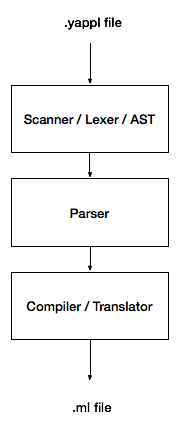
\includegraphics[width=1.5in]{block-diagram.png}

\subsection{Components}
\subsubsection{Symbol Table}
The translator builds an initial table for storing user specified identifiers and their type. The table can also point to a parent table, allowing for scoping. This scoping occurs, for example, in a declaration of a \term{(} \nterm{pattern} \term{::} \nterm{pattern} \term{)} match. To detect a problematic pattern such as  \term{(a::a)}, the first \term{a} is added to a blank symbol subtable. When converting the second \term{a} into output, the compiler will notice that an \term{a} has already been created in the subtable and raise an error. 
\subsubsection{expr\_to\_string} 
This is the main function for the evaluation of the program expression and returns both a string representation of the parse tree it is given, and its type. It is called recursively to evaluate the program parse tree. As part of the output generation, types are checked for validity. When the function converts identifiers to strings, it will first check if that identifier is built-in, such as \texttt{print}, before performing a lookup with the symbol table.
\subsubsection{Memoization}
Memoization is implemented using a hash table that is populated when a memoized function is called with a new parameter.  In the generated code, all user-defined identifiers (not just those in the memoized function) will be prepended with \texttt{yappl\_}, to prevent namespace collisions with OCaml identifiers, such as hash tables, used by the YAPPL compiler.
\subsubsection{Compiling to executable}
The \texttt{ocamlc} utility links the compiled generated code with built-in OCaml functionality such as \texttt{rand}. It also prepends \texttt{stdlib.ypl}, if it exists, to function as a standard library.
\newpage

\section{Test Plan}
\subsection{Example Programs}
Todo. Show two sample programs with .ml output.\\

\subsection{Test Suites}
Todo. Show tests. Explain how and why they were chosen. Explain what kind of automation was used. Say who did what.\\
\newpage

\section{Lessons Learned}
David. Todo.\\

Jonathan. Todo.\\

Hans. Todo.\\

Harley. Todo.\\

\subsection{Advice for the Future}
Todo.\\
\newpage

\section{Appendix}
%lstset{language={[Objective]Caml}}
\lstinputlisting[title=ast.ml]{../yappl/ast.ml}
\lstinputlisting[title=builtin.ml]{../yappl/builtin.ml}
\lstinputlisting[title=builtin.mli]{../yappl/builtin.mli}
\lstinputlisting[title=parser.mly]{../yappl/parser.mly}
\lstinputlisting[title=scanner.mll]{../yappl/scanner.mll}
\lstinputlisting[title=translate.ml]{../yappl/translate.ml}
\lstinputlisting[title=yappl.ml]{../yappl/yappl.ml}

\lstinputlisting[title=errors.sh, language=bash]{../yappl/errors.sh}
\lstinputlisting[title=Makefile, language=bash]{../yappl/Makefile}
\lstyappllisting{stdlib.ypl}
\lstinputlisting[title=testall.sh, language=bash]{../yappl/testall.sh}
\lstinputlisting[title=yapplc, language=bash]{../yappl/yapplc}

\lstset{language=YAPPL}
\lstyappllisting{tutorials/add.ypl}
\lstyappllisting{tutorials/dpmem.ypl}
\lstyappllisting{tutorials/geom.ypl}
\lstyappllisting{tutorials/geom-cond.ypl}
\lstyappllisting{tutorials/memogeom.ypl}

\lstyappltestlisting{test-array-cons}
\lstyappltestlisting{test-basic-operators}
\lstyappltestlisting{test-binding}
\lstyappltestlisting{test-functions}
\lstyappltestlisting{test-list-indexes}
\lstyappltestlisting{test-memo}
\lstyappltestlisting{test-more-operators}
\lstyappltestlisting{test-pattern-matching}
\lstyappltestlisting{test-pattern-matching-elist}
\lstyappltestlisting{test-pattern-matching-bug1}
\lstyappltestlisting{test-pattern-matching-bug2}
\lstyappltestlisting{test-print-line}

\lstyappllisting{errors/boolBindPLUSint.ypl}
\lstyappllisting{errors/boolIndex.ypl}
\lstyappllisting{errors/floatIndex.ypl}
\lstyappllisting{errors/intBindMINUSfloat.ypl}
\lstyappllisting{errors/intBindPLUSfloat.ypl}
\lstyappllisting{errors/intORint.ypl}
\lstyappllisting{errors/intPLUSfloat.ypl}
\lstyappllisting{errors/notAnERror.ypl}
\newpage

\end{document}